\chapter{Summary and Comparison of Existing Learning Based Models}

\label{appendix:models}

\section{DeepPE}

Developed by Kim et al, DeepPE is one of the earliest attempt at predicting the outcomes of prime editing using machine learning and illustrated many possible determinants of PE efficiency. Most of the determinants discovered in their study are still valid today, but the model itself is not as relevant in terms of performance due to the constraints in datasets at the time of their publication. The model is also very limited in terms of editing types supported, focusing on predicting the efficiency of G to C substitution at the position +5 nick site of the target sequence. 

After the users provided the target sequence to edit, the web tool will propose a number of pegRNA sequences and evaluate their efficiency using the DeepPE model. The 47-nt long target sequence and the 17 to 37nt RTT+PBS sequences, as well as 20 explicit features including the GC content and melting temperature of the PBS are used as input to the model. The two nucleotide sequences are one-hot encoded into four dimensional matrices. The two embedded sequences and the explicit features are then concatenated(stacked) together and fed into a convolutional neural network with 10 $3 \times 4$ filters. The output is pooled using a deep reinforcement learning model instead of a traditional pooling layer, and then input into a fully connected layer with 1000 units. The result is linearly transformed to the DeepPE prediction score, indicating the efficiency of the editing process on the target sequence using the provided PBS and RTT.

A sketch of the model architecture is shown in \autoref{fig:deeppe}.

\begin{figure}[ht]
    \centering
    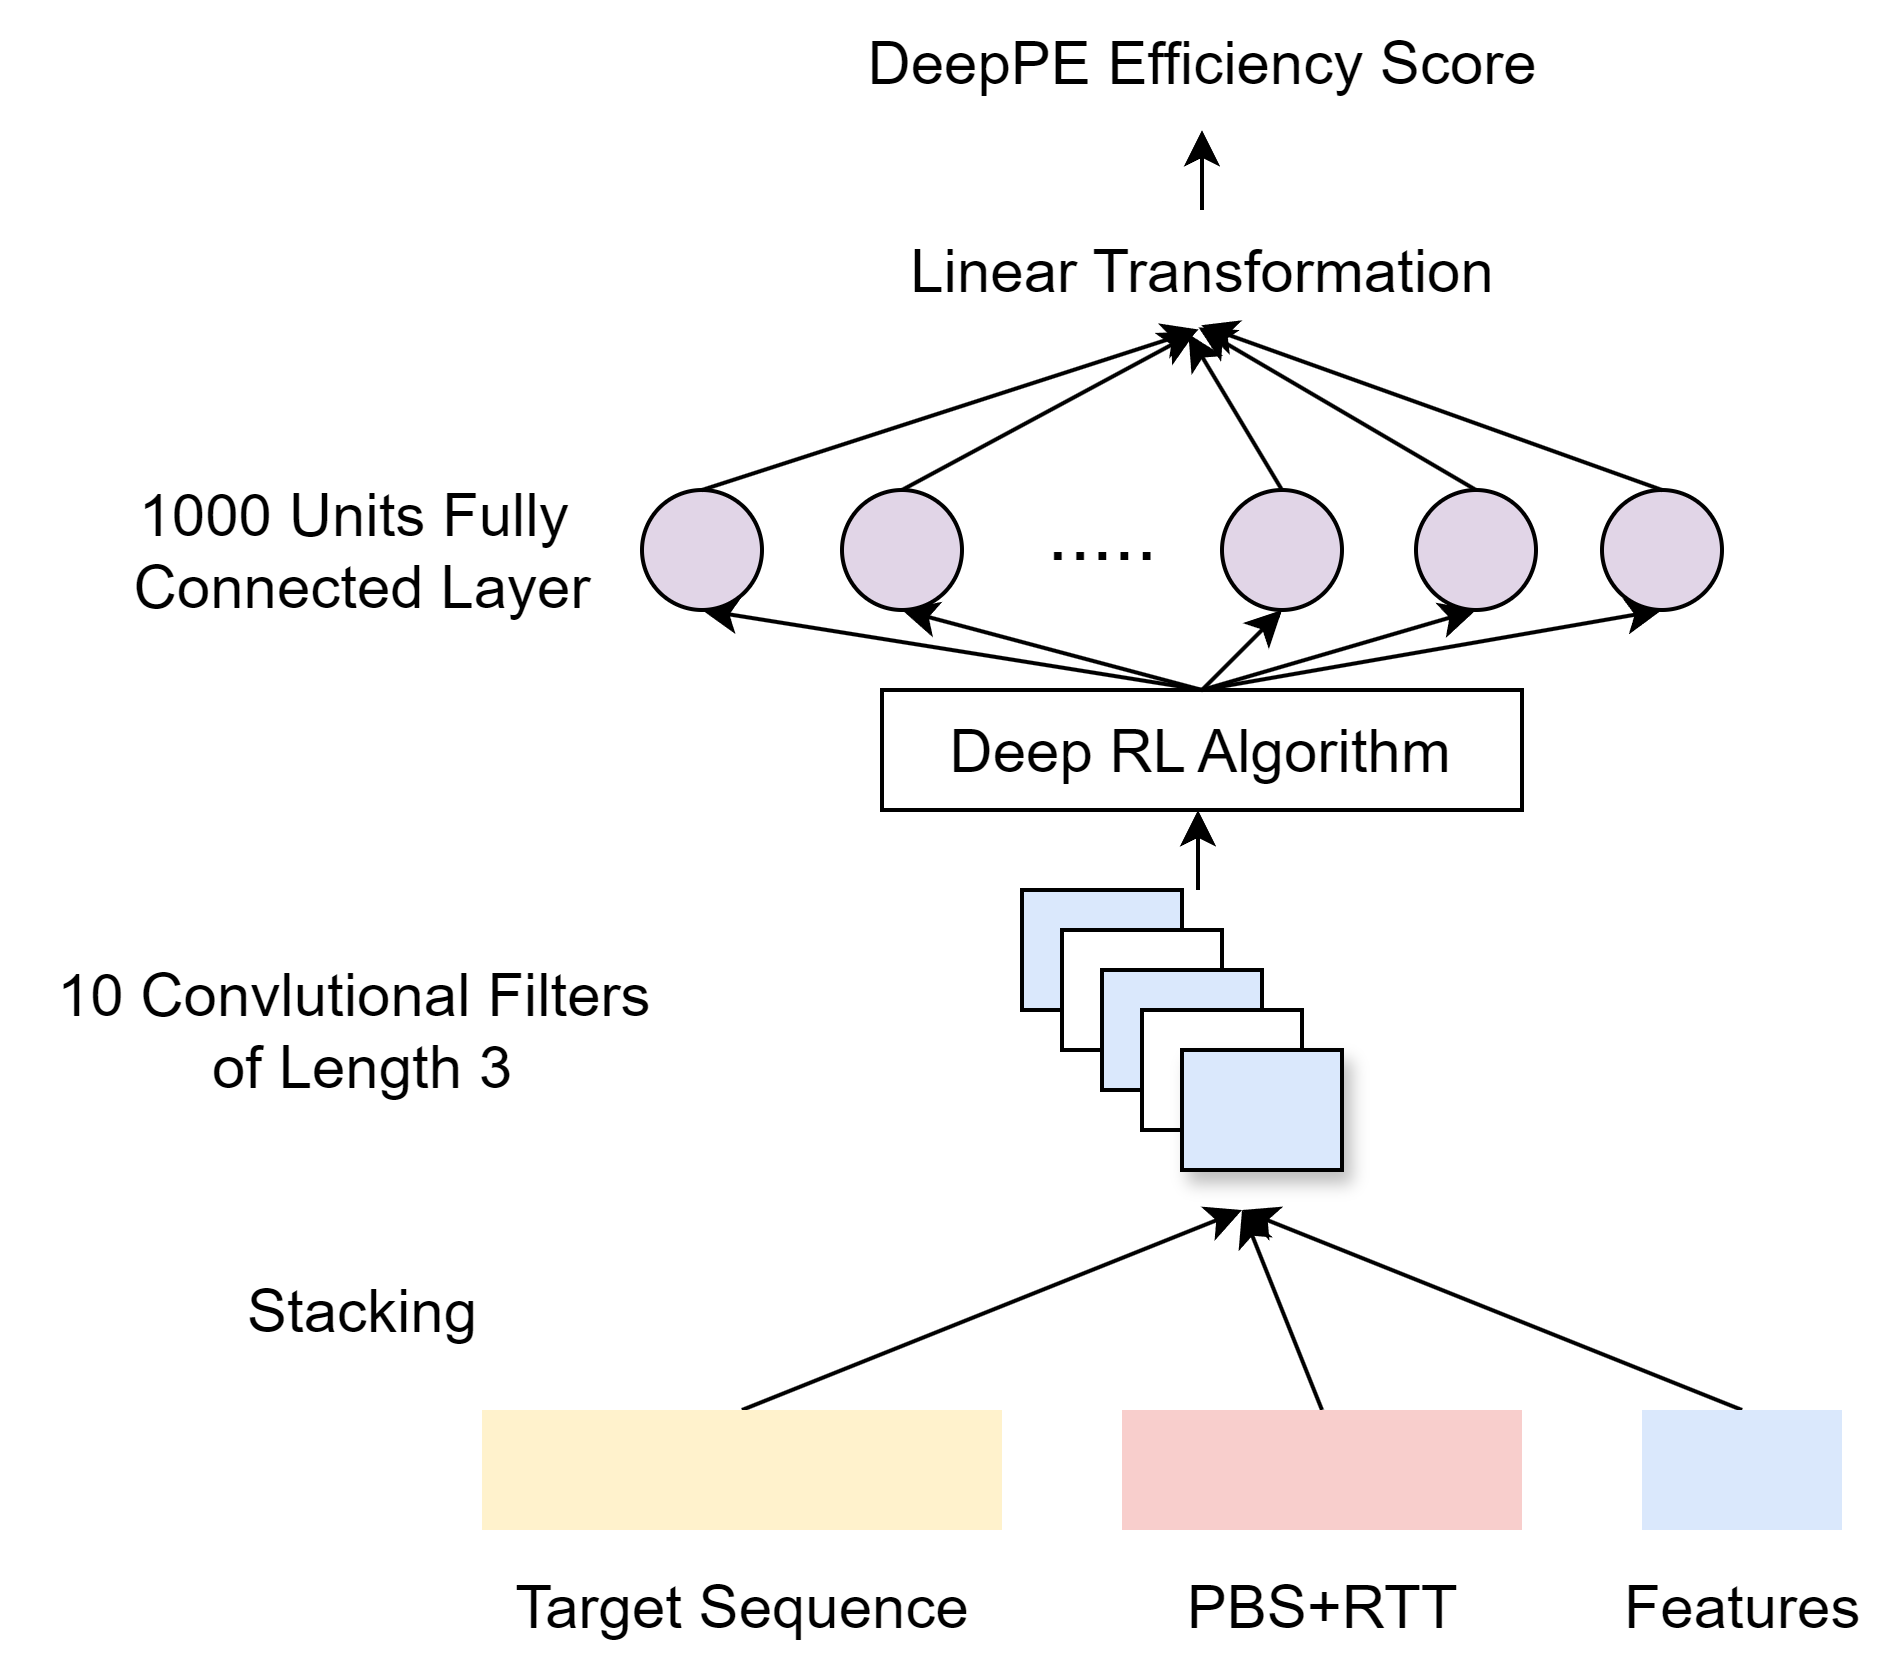
\includegraphics[width=0.6\textwidth]{DeepPE.png}
    \caption{DeepPE Model Architecture}
    \label{fig:deeppe}
\end{figure}

This architecture had the highest performance among the methods reviewed by the authors, although not significantly higher than L1 Lasso regression model. The model achieved a Spearman's R of 0.7 to 0.8, and a Pearson's r of 0.6 to 0.7 on the held-out as well as generalization(unseen) datasets.

The authors also developed another multi-layer perceptron(MLP) model to predict the editing efficiency of more general editing types, including single-nucleotide insertions, deletions and substitutions. However, random forest achieved better performances and was thus used in the additional PE\_Type and PE\_Position models. PE\_Type model proposes pegRNA for 24 possible edits, including specific single-nucleotide deletions, insertions, and substitutions at designated locations. PE\_Position model proposes pegRNA optimized to perform substitutions at ten more positions, namely positions 1, 2, 3, 4, 6, 7, 8, 9, 11 and 14.

\section{Easy Prime}

EasyPrime is a XGBoost regression model developed by Liu et al to produce design for RTT, PBS and ngRNA. Instead of arbitrary mutations, Easy-Prime predicts the editing efficiency of the variants logged in the Genome-Wide Association Studies(GWAS) database. The GWAS variants are the single nucleotide polymorphisms(SNPs) that have been associated with particular traits or diseases.

Similar to DeepPE, for each variant, the web tool proposes a number of pegRNA design using the constrains on PBS, RTT and ngRNA length provided by the user. The proposed pegRNAs are then evaluated by the XGBoost models to find the optimal candidate. When producing the efficiency score, EasyPrime takes the extracted features from pegRNA and target sequences as input to the model instead of the sequences themselves. The extracted features include GC content of the PBS, PAM sequence disruption, as well as several target mutation features describing the mutations to insert.

Cas9 activity score produced by DeepSpCas9 is also used as a feature in the model. DeepSpCas9 is a convolutional neural network model that predicts the activity of the SpCas9 protein on a given target sequence and sgRNA pair. The model architecture is very similar to DeepPE, with one convolutional layer followed by three fully connected layers. The unique feature of the model is the use of filters of different sizes in the convolutional layer(3, 5, and 7nt), allowing the model to capture the dependencies between the base pairs at different distances\cite{kimSpCas9ActivityPrediction2019}.

Albeit limited in the type of edits supported, EasyPrime is one of a few methods that provides official support for ngRNA design required by PE3 and PE3b. Note that PE3b is the optimized version of PE3, where the ngRNA is selected to avoid possible DSB by not targeting the nucleotide complementary to the nicked position\cite{liudavidr.SearchandreplaceGenomeEditing2019}.

Constrained by the data available and the simple architecture of the model, the performance of EasyPrime is relatively low compared to the other models reviewed. The model achieved a Spearman's R and Pearson's r of 0.5 to 0.6 on their held-out datasets.

\section{DeepPrime}

\begin{figure}[ht]
    \centering
    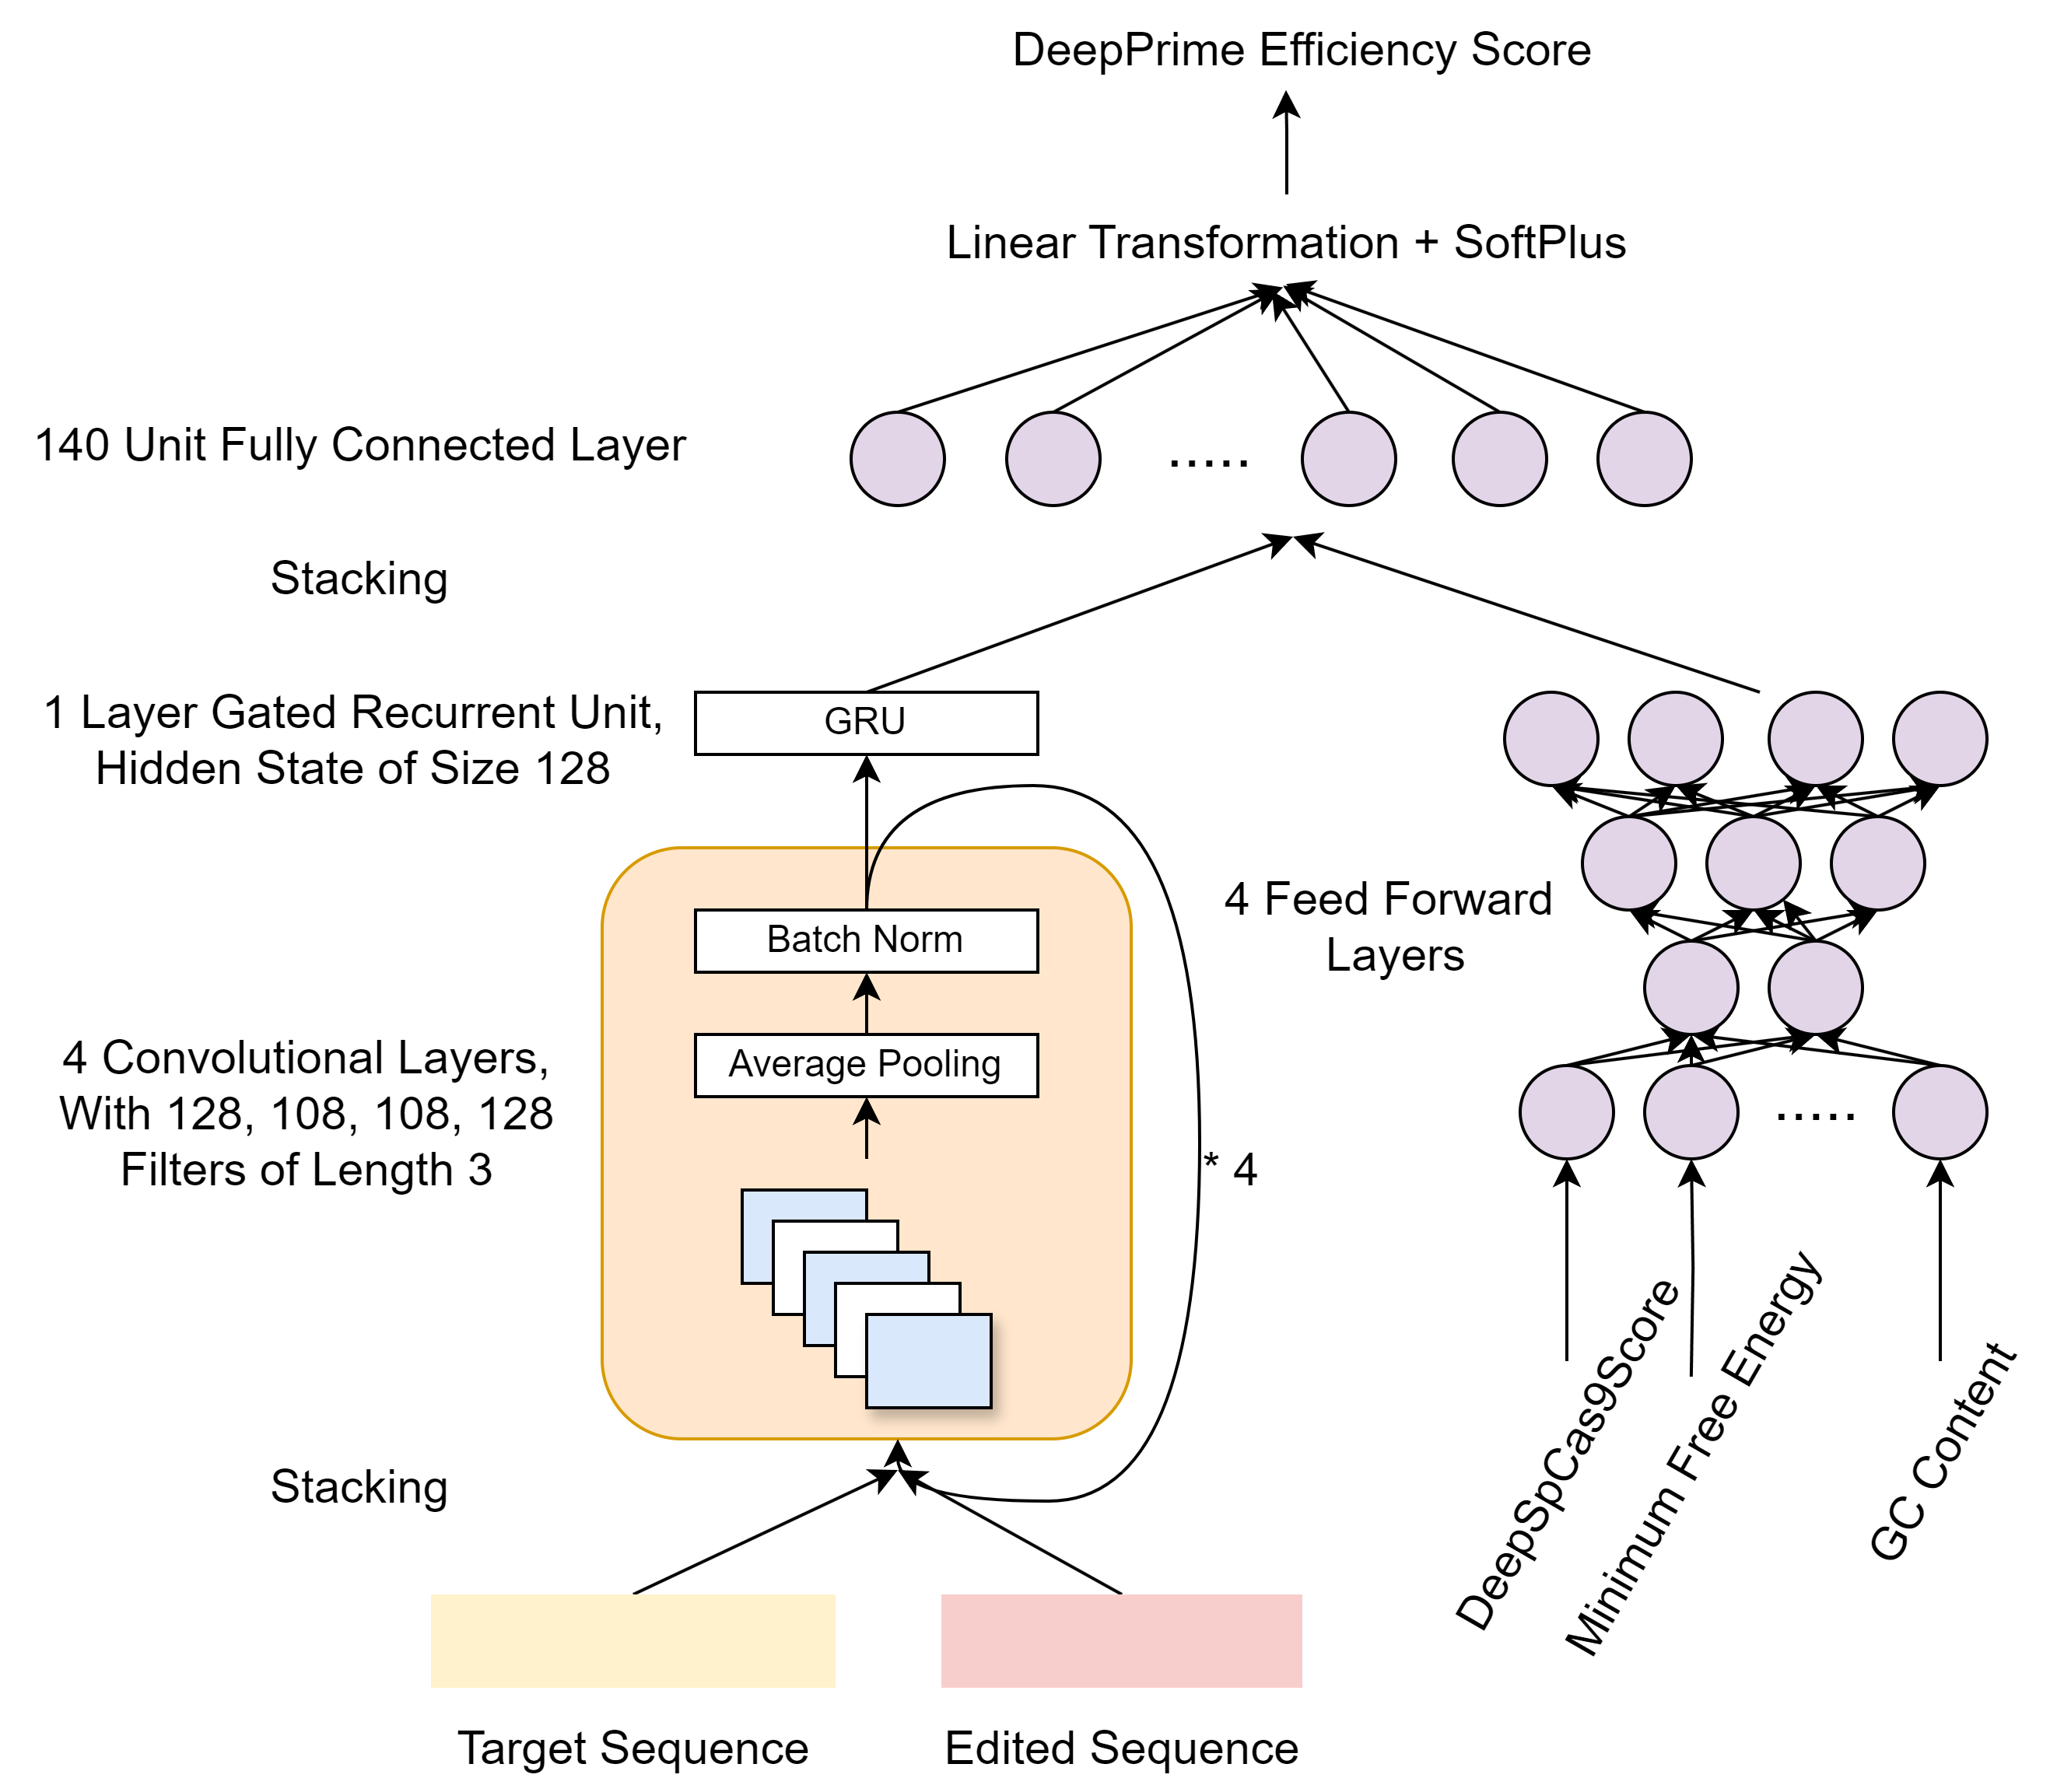
\includegraphics[width=0.8\textwidth]{DeepPrime.png}
    \caption{DeepPrime Model Architecture}
    \label{fig:deepprime}
\end{figure}


Also developed by Kim et al., DeepPrime is the updated version of DeepPE with an upgraded model architecture. 

Illustrated in \autoref{fig:deepprime}, instead of PBS + RTT with target sequence, it takes the wild type(unedited) as well as the edited sequences as input to the CNN. The convolutional network is significantly larger than DeepPE, containing four convolutional layers with 128, 108, 108, and 128 filters, respectively. Moreover, conventional average pooling is used this time round after each convolutional layer instead of a deep RL algorithm. Batch normalization is also applied to accelerate training.  The output of the convolutional layer is then processed by bidirectional Gated Recurrent Units(GRU). 

Instead of processed together with the embedded sequence, features extracted from the proposed pegRNA and target context sequence are processed using a separate four-layer feed forward neural network. The outputs from the two networks are then stacked and fed into a fully connected layer. The result is linearly transformed and processed by a SoftPlus activation function to produce the final prediction score.


DeepPrime is effectively a multi-task learning model, with a base model trained using the combination of 18 datasets of different PE and cell line combinations. The base model is then fine tuned using each of the 18 datasets to produce a task specific model for each setting, collectively named DeepPrime-FT.  

The amount of training data used makes DeepPrime the most comprehensive method in terms of the number of cell lines and PE versions covered. At the same time, the multi-task design allows DeepPrime-FT to utilize the share features between the different PEs and cell lines, and thus achieve very high performance. 

The model has made significant improvement compared to DeepPE, with a Spearman's R of 0.8 to 0.9, and a Pearson's r of 0.7 to 0.9 on most of the testing datasets, including the generalization datasets unseen during training.

\section{PRIDICT}

\begin{figure}[ht]
    \centering
    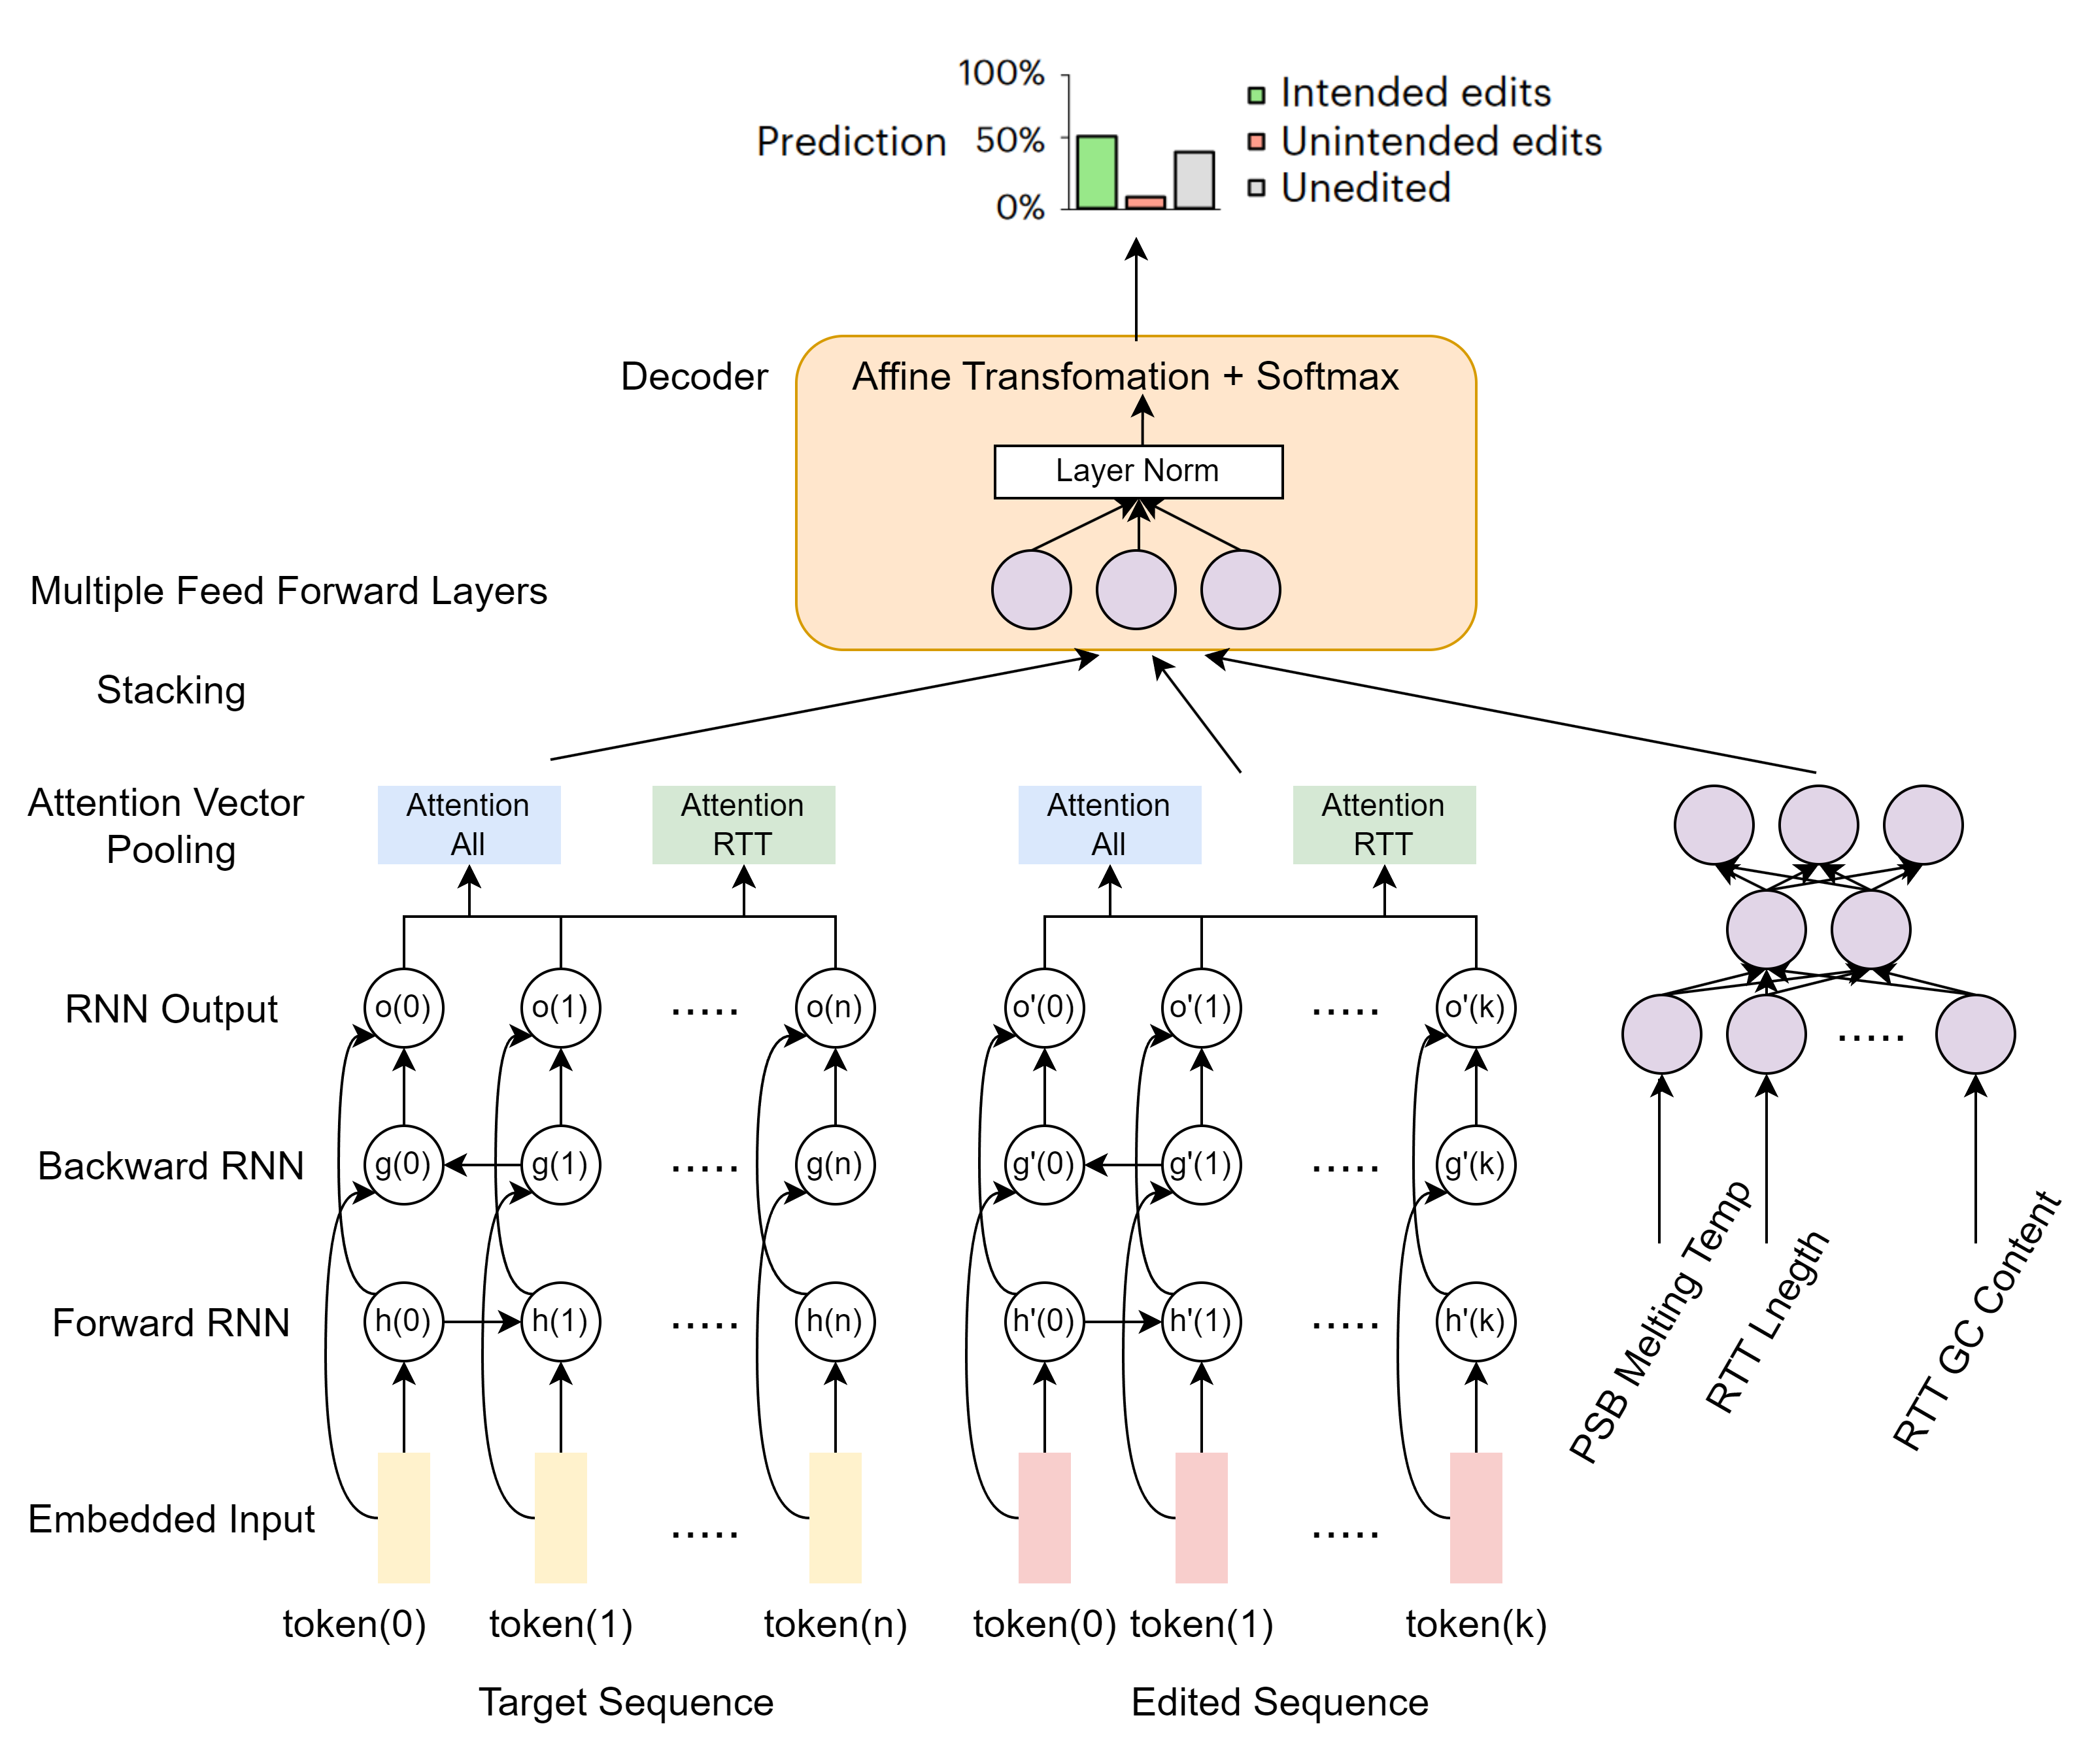
\includegraphics[width=\textwidth]{pridict.png}
    \caption{PRIDICT Model Architecture}
    \label{fig:pridict}
\end{figure}


Developed by Gerald Schwank et al, PRIDICT utilizes a sophisticated attention-based bidirectional RNN model with a similar pegRNA recommendation pipeline to DeepPE and DeepPrime. 

The model overall is a three encoder one decoder architecture. Two of the encoders are attention-based bidirectional RNN models, learning the vector representation of the sequence data. The third encoder is a feed forward neural network taking explicit features derived from the proposed pegRNA, such as the length of the modifications to insert and melting temperature of the PBS, as inputs, similar to DeepPrime.

The target and mutation sequences are one-hot encoded, alongside three additional binary encoding indicating whether the nucleotide belongs to the protospacer, RTT or PBS. The four embeddings are stacked together into a vector of length 9 for each token in the target sequence and 7 for the mutated sequence(the protospacer embedding is omitted for mutated sequence) and fed into the model.

The bidirectional RNN model is used to capture the dependencies between the base pairs within the whole sequence, instead of only past information captured by unidirectional RNN models. Two separate attention query vectors then pools(compresses) sequence of token-level representations into one fixed length vector using the calculated attention weights. One query vector pools all tokens of the sequences, providing context. The other pools only RTT tokens, focusing on the part where the edits are made. 

The decoder is another feed forward neural network with residual connections and layer normalization, taking the pooled vectors from the encoders and calculating the probability distribution of possible outcomes of the edits when using the proposed guide. 

The model architecture is illustrated in \autoref{fig:pridict}.

Significantly higher performance was achieved by PRIDICT when compared to DeepPE (including PE\_Type and PE\_Position) and EasyPrime, with 2-3 fold increase in Spearman's R and Pearson's r on the generalization datasets curated by Gerald et al. PRIDICT also achieved comparable or better results on the datasets DeepPE and EasyPrime were originally trained on. In terms of current generation of models, it was on par with DeepPrime on the HEK293T datasets when predicting intended edits, with a Spearman's R of 0.81. At the same time, PRIDICT outperformed the MinsePIE model as mentioned in section \ref{sec:minsepie}.
